\documentclass[10pt,conference]{IEEEtran}

%\usepackage[utf8]{inputenc}\usepackage[T1]{fontenc}
\usepackage{titling}
%\usepackage{times}
\setlength{\droptitle}{-5em}   % This is your set screw
\usepackage{ps2}
\usepackage{comment}
\usepackage{physics}
\usepackage{setspace}
\usepackage{bbm}
\usepackage{algorithm}
\usepackage{algorithmic}
\usepackage{etoolbox}
\AtBeginEnvironment{algorithm}{%
	\setlength{\columnwidth}{\linewidth}%
}
%\usepackage{titlesec}
%\titleformat{\section}{\large\bfseries}{\thesection}{1em}{}
\DeclareMathOperator{\interi}{int}
\DeclareMathOperator{\Clip}{clip}

\title{\bf\Large{Multi-Agent Area Coverage Control Using Reinforcement Learning}}
\author{Simon Hu}

\begin{document}
	
\maketitle
\thispagestyle{empty}
\pagestyle{empty}
\begin{abstract}
	In this paper, an area coverage control law is combined with a reinforcement learning algorithm to solve the optimal deployment problem. Traditional methods proposed for solving the method, from classical control theory, use proportional or linear quadratic Gaussian control designs. These traditional methods lack the robustness and adaptivity to dynamic environments, especially when these dynamic environment contribute significantly to the motion of the agents. A delayed actor-critic deep deterministic policy gradient algorithm is proposed to learn the value function and optimal policy. Simulation results are presented for stationary and time-varying scalar fields.
\end{abstract}
\section{Introduction}
	Coverage control of multi-agent system is concerned with deploying agents over an environment to maximize sensor coverage, for various tasks such as sensing, data collection and surveillance missions. Applications of this problem are harbour patrol, search and rescue, data, and surveillance missions. Consider a group of $N$ homogeneous agents moving in a compact environment $\Omega \subset \R^2$, where the dynamics of the $i$-th agent are given by 
	\begin{equation}
		\label{dynamics}
		\displaystyle \dot{p}_i = u_i
	\end{equation}
	where $p_i = (x_i, y_i)$ represents the agent's location and $u_i = (u_{x_i}, u_{y_i})$ represents the control input, which in this case is the direct velocity input. The goal of solving the coverage control problem is to find the configuration of agent positions $p = (p_1, p_2, \dots, p_N)$ such that the cost index 
	\begin{equation}
		\label{cost index}
		\displaystyle \mathcal{H}(p,t) = \int_{\Omega}{\max\limits_{i=1,2,\dots,N}{f_i(\,\norm{q - p_i})}\phi(q,t) \: \dif q}
	\end{equation}
	is maximized. In the above, $\phi : \Omega \times \R_{\geq 0} \to \R_{\geq 0}$ is a probability density that represents the probability of an event occuring at point $q \in \Omega$ and $f: \R^2 \to \R$ is a non-increasing function. The integral is understood in the sense of Lesbegue. Intuitively, the spread of $\phi$ reflects a measure of the number of agents to be deployed in that area. This density is assumed to be known, or computed externally. The choice of $f$ reflects the type of coverage task we are attempting. For the maximum area coverage problem, the function $f(x) = -x^2$ is considered. It is easily checked that $f$ is measurable on $\Omega$ and is a non-increasing function. 
	\subsection{Voronoi Tesselations}
		A collection $S = (S_1, S_2, \dots, S_M)$ is a partition of $\Omega$ if $\interi(S_i) \cap \interi(S_j) = \emptyset$ (i.e. the sets have disjoint interiors) and $\cup(S_i) = \Omega$ (i.e. the union of the sets completely cover $\Omega$). We consider a particularly special partition of the space called the Voronoi partition. The Voronoi partition of $\Omega$ is given by $\V_\Omega = (\V^1, \V^2, \dots, \V^N)$ where each $\V^i$ is described by 
		\begin{equation}
			\label{voronoi partition}
			\displaystyle \V^i = \left\{ q \in \Omega \, | \, \norm{q - p_i} \leq \norm{q - p_j}, \, \forall j \neq i \right\}.
		\end{equation}
		Agents $i$ and $j$ are Voronoi neighbors if they share a boundary. That is, 
		\begin{equation*}
			\displaystyle \partial \V^i \cap \partial \V^j \neq \emptyset.
		\end{equation*}
		The mass and center of mass of a Voronoi cell are given by 
		\begin{equation*}
			\displaystyle m_{\V^i} = \int_{\V^i}{\phi(q,t) \: \dif q}, \:\: c_{\V^i} = \frac{1}{m_{\V^i}}\int_{\V^i}{q\phi(q,t) \dif q}
		\end{equation*}
		respectively. 
		\begin{figure}
			\begin{subfigure}{0.2\textwidth}
				\centering 
				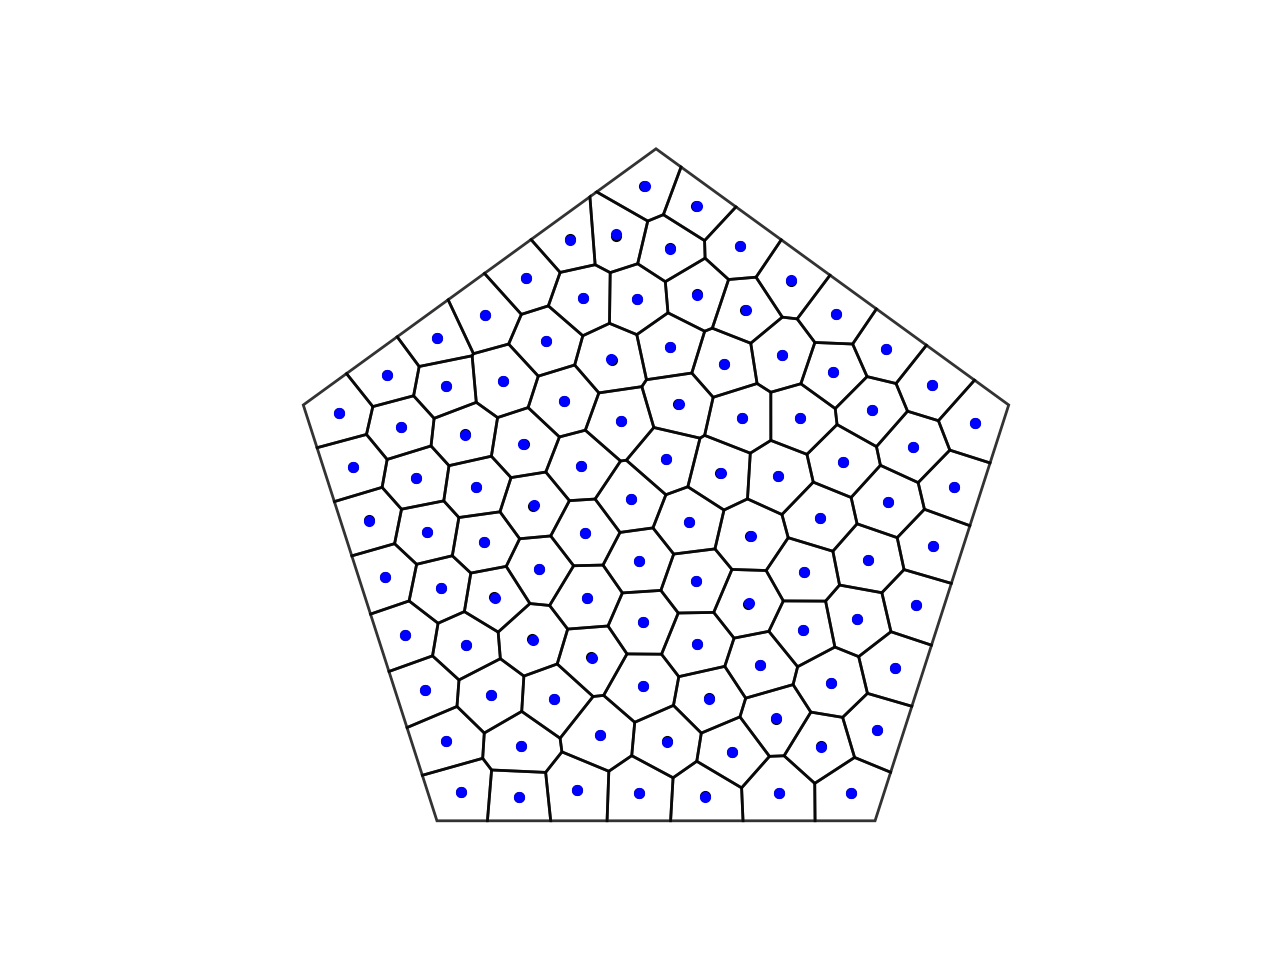
\includegraphics[scale=0.2]{fig_ex_2}
				\caption{}
			\end{subfigure}\hspace{\fill}
			\begin{subfigure}{0.2\textwidth}
				\centering 
				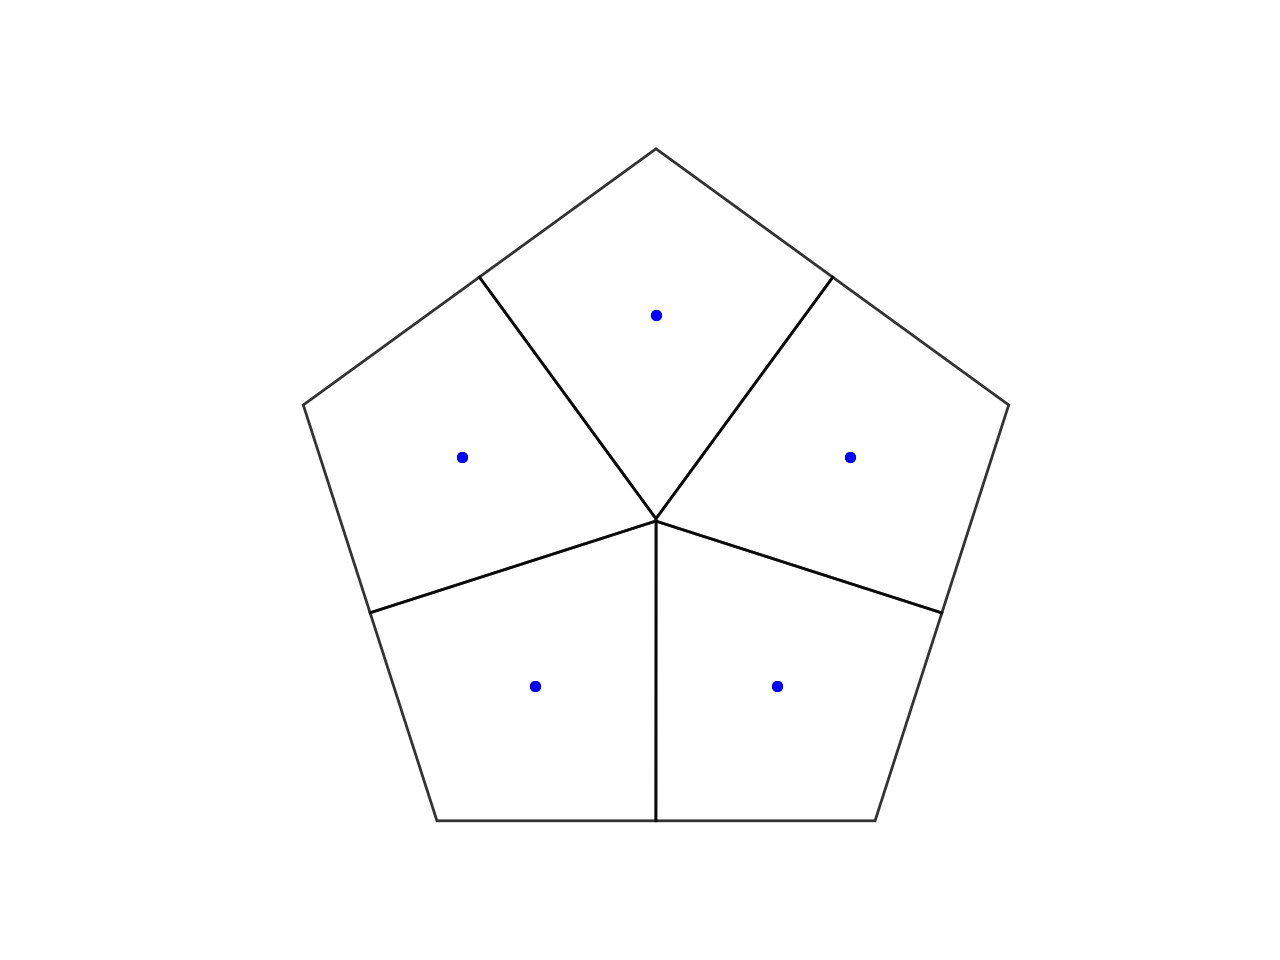
\includegraphics[scale=0.2]{fig_ex}
				\caption{}
			\end{subfigure}
			\caption{(a) A Voronoi tesselation assuming that $\phi(q,t) = 1$. (b) A centroidal Voronoi tesselation assuming that $\phi(q,t) = 1$.}
		\end{figure}
		\begin{prop}
			Under the Voronoi partition, the cost index (\refeq{cost index}) can be rewritten as
			\begin{equation}
				\label{rewritten cost index}
				\displaystyle \mathcal{H}(p,t) = \sum\limits_{i=1}^{N}{\int_{\V^i}{f(\,\norm{q - p_i})\phi(q,t) \dif q}}.
			\end{equation}
		\end{prop}
		\begin{proof}
			Since $\V_\Omega$ is a covering of $\Omega$, we write (\refeq{cost index}) as 
			\begin{equation*}
				\displaystyle \mathcal{H}(p,t) = \sum\limits_{i=1}^{N}{\int_{\V^i}{\max\limits_{i=1,2,\dots,N}{f_i(\,\norm{q - p_i})}\phi(q,t) \: \dif q}}.
			\end{equation*}
			The result then follows by the non-increasing nature of $f$ and the definition of $\V^i$.
		\end{proof}
		This form of the cost function implies that agent $i$ only needs local information to compute its contribution to the total cost. As such, the algorithm is called spatially distributed, with respect to the Voronoi tesselation. 
		
		The implications proposition 1 are far reaching. Consider a scenario where agents must communicate with each other to obtain location information, for the purpose of avoiding collisions. Communications can be energy-intensive or unreliable as the distance between agents is large, but proposition 1 says that agent $i$ only needs to communicate with its Voronoi neighbors which reduces the burden on communications. 
	\subsection{Optimal Policy}
		It is shown in \cite{Cortes:2004} that the optimal partition of $\Omega$ is the centroidal Voronoi partition and the optimal sensor placements $p$ are the centers of the Voronoi cells. As such, our goal is to find controls $u_i$ that drive the agents towards their Voronoi centroids. In \cite{Cortes:2004}, the authors consider a simple proportional-derivative controller of the form 
		\begin{equation*}
			\displaystyle u_i = -k_p(c_{\V^i} - p_i) - k_d(\dot{c}_{\V^i} - \dot{p}_i)
		\end{equation*}
		which performs reasonably well. However, many classical control methodologies have to tune hyperparameters or use some sort of integral control to account for different inputs. Reinforcement learning methods are introduced to train agents that can adapt to changing environments. This is especially important in scenarios where agents are deployed over hydro or aerodynamic environments.  
\section{Actor-Critic Neural Network}
	Designing a controller that realizes the control law in \cite{Cortes:2004} is difficult even for simple dynamics. When the dynamics become more complex, like an underwater glider for example, the controller design becomes more intricate and complicated. Reinforcement learning methodologies are introduced to reduce this burden. To this end, an Actor-Critic neural network approximation is employed. Define $e_i(t) = c_{\V^i}(t) - p_i(t)$ as the centroid error for agent $i$ and consider the Value function at the $k$-th step, given by 
	\begin{equation}
		\label{value function}
		\displaystyle V(e_i(k)) = \sum\limits_{\kappa = k}^{\infty}{e_i^T(\kappa)Qe_i(\kappa) + u_i^T(\kappa)Ru_i(\kappa)}
	\end{equation}
	where $Q, R \in \R^{2 \times 2}$ are positive definite matrices. If we consider a Gaussian process for the noise then this is just the linear quadratic regulator from classical controls. The second term in the Value function encodes a measure of energy expenditure for physical systems, so the design of the $R$ matrix is important for long-term surveillance and data collection tasks. For notational simplicity, let us write $V_{i,k} = V_i(e(k))$. The Value function is rewritten in the form of a Bellman equation, 
	\begin{equation}
		\displaystyle V_{i,k} = e_i^T(k)Qe_i(k) + u_i^T(k)Ru_i(k) + V_{i,k+1}
	\end{equation}
	so that the minimization problem to be solved is
	\begin{equation}
		\displaystyle V_{i,k}^* = \min\limits_{}{\left[ e_i^T(k)Qe_i(k) + u_i^T(k)Ru_i(k) + \gamma V_{i,k+1}^* \right]}
	\end{equation}
	where $\gamma$ is the discount factor. The goal is to find the optimal policy $\pi_i = u_i$ that minimizes the Value function. To solve the problem, the authors in \cite{FLAIRS1612802} use a neural network to approximate the Value function and the policy. The assumed structure of both functions are given by 
	\begin{equation}
		\displaystyle \widehat{V}_j(e_i(k)) = \omega_{c,j}^T\rho(e_i(k)),
	\end{equation}
	\begin{equation}
		\displaystyle \widehat{\pi}_{j}(e_i(k)) = \omega_{a,j}^T\sigma(e_i(k)).
	\end{equation}
	In the above, $\widehat{V}_j$ and $\widehat{\pi}_j$ are the estimates of the Value function and policy respectively, $\omega_{c,j}, \omega_{a,j}$ are the network weights at iteration $j$, and $\rho, \sigma$ are a series of activation functions from the network. The authors of \cite{FLAIRS1612802} consider a least-squares loss for both the actor and critic, but we will use the MSE loss instead, given by
	\begin{equation}
		\label{critic_loss}
		\displaystyle E_{c,j} = \frac{1}{N_t}\sum\limits_{\ell=1}^{N_t}{\left[ \omega_{c,j+1}^T\rho^\ell(e_i(k)) - V_{i,j+1}^\ell \right]}
	\end{equation}
	\begin{equation}
		\label{actor_loss}
		\displaystyle E_{a,j} = \frac{1}{N_t}\sum\limits_{\ell=1}^{N_t}{\left[ \omega_{a,j+1}^T\sigma^\ell(e_i(k)) - \pi_{i,j+1}^\ell \right]}.
	\end{equation}
	A target and source network are initialized and tracked for both the actor and critic. The weights are synched using a soft-update rule to improve numerical stability. A vanilla actor-critic DDPG algorithm is given by Algorithm \refeq{acddpg}.
	\begin{algorithm}
		\caption{Actor-Critic DDPG}
		\begin{algorithmic}[1]
			\STATE Randomly initialize the critic network $Q(s, a|\theta^Q)$ and actor network $\pi(s|\theta^\mu)$ with weights $\theta_Q, \theta^\pi$. 
			\STATE Initialize a target network $Q'$ and $\pi'$ with the same weights as the networks above. 
			\STATE Initialize an empty replay buffer $R$.
			\FOR {episode = 1 \TO M} 
				\STATE Initialize a random process $\mathcal{N}$ for exploration. 
				\STATE Obtain an initial observation of the state, $s_1$. 
				\FOR {t = 1 \TO T}
					\STATE Select action $a_t = \pi(s_t|\theta^\mu) + \mathcal{N}_t$ according to the current policy and exploration noise.
					\STATE Execute action $a_t$ and observe the reward $r_t$ and new state $s_{t+1}$. 
					\STATE Store the transition dictionary $(s_t, a_t, r_t, s_{t+1})$ to $R$.
					\STATE Sample a minibatch of $N$ transitions $(s_i, a_i, r_i, s_{i+1})$ from $R$.
					\STATE Set $y_i = r_i + \gamma Q'(s_{i+1}, \pi'(s_{i+1}|\theta^{\pi'})|\theta^{Q'})$. 
					\STATE Update the critic network by minimizing the loss, given by equation (\refeq{critic_loss}).
					\STATE Update the actor network using the sampled policy gradient given by 
					\begin{equation*}
						\displaystyle \nabla_{\theta^\pi} J \approx \frac{1}{N}\sum\limits_{i}{\nabla_a Q(s,a|\theta^Q)|_{s - s_i, a = \pi(s_i)}\nabla_{\theta^\pi}\pi(s|\theta^\pi)|_{s_i}}.
					\end{equation*}
					\STATE Perform a soft update of the target networks:
					\begin{align*}
						&\theta^{Q'} \leftarrow \tau\theta^Q + (1-\tau)\theta^{Q'} \\
						&\theta^{\pi'} \leftarrow \tau \theta^\pi + (1-\tau)\theta^{\pi'}
					\end{align*}
				\ENDFOR
			\ENDFOR
		\end{algorithmic}
		\label{acddpg}
	\end{algorithm}
\section{Twin-Delayed Soft-Actor Critic DDPG}
The Soft Actor-Critic DDPG Algorithm suffers from the overestimation of the value function, which propagates throughout learning and can negatively affect the learned policy. This motivates the development of double $Q$-learning algorithms where the action selection and $Q$-value updates are decoupled through the use of two value networks. In the setting of DDPG, we have two deterministic actors $\pi_{\theta_1}, \pi_{\theta_2}$ and two corresponding critics $Q_{\omega_1}, Q_{\omega_2}$ so that the Bellman update is given by 
\begin{align*}
	\displaystyle &y_1 = r + \gamma Q_{\omega_2}(s', \pi_{\theta_1}(s')), \\
	&y_2 = r + \gamma Q_{\omega_1}(s', \pi_{\theta_2}(s')).
\end{align*}
Then clipped double $Q$-learning is applied, which uses the minimum estimated update between the two above so that we trend towards an underestimation. This bias towards the underestimation is much harder to propagate through training. Furthermore, the authors in \cite{fujimoto2018addressing} consider a delayed soft update of the network parameters. The reasoning for this is that the policy and value updates are coupled and value function estimates diverge when the estimate of the policy is poor. Conversely, the policy will be poor if the value estimate is inaccurate. As such, to reduce this variance the authors of \cite{fujimoto2018addressing} updates the policy at a lower frequency than the $Q$-function. This promotes stability of the network and improves the numerical accuracy of the results. Finally, the authors of \cite{fujimoto2018addressing} add a regularization parameter for smoothing. To achieve this, small amounts of clipped random noise are added to the action and minibatches are used. With this clipping, the Bellman update becomes 
\begin{equation*}
	\displaystyle y = r + \gamma Q_\omega(s', \pi_{\theta}(s') + \epsilon), \:\: \epsilon \sim \Clip(\mathcal{N}(0, \sigma), -c, +c).
\end{equation*}
The twin-delayed actor-critic DDPG (TD3) algorithm is given in Algorithm (\refeq{sacddpg}). The proposed area coverage control algorithm is then given by combining the TD3 algorithm to find the optimal policy and the Voronoi partitions are used to find the centroid, which is the point the agent must move towards. 
\begin{algorithm}
	\caption{Twin-Delayed Actor-Critic DDPG}
	\begin{algorithmic}[2]
		\STATE Initialize critic networks $Q_{\omega_1}, Q_{\omega_2}$ and actor network $\pi_{\theta}$ with random parameters
		$\omega_1, \omega_2, \theta$. 
		\STATE Initialize the target networks $\omega'_1 \leftarrow \omega_1, \omega'_2 \leftarrow \omega_2, \theta' \leftarrow \theta$.
		\STATE Initialize a replay buffer $R$.
		\FOR {$t = 1$ \TO $T$}
			\STATE Select action with exploration noise $a \sim \pi(s) + \epsilon, \epsilon \sim \mathcal{N}(0, \sigma)$ and record the reward $r$ and new state $s'$. 
			\STATE Store the tuple $(s, a, r, s')$ into $R$. 
			\STATE Sample minibatches of $N$ transitions $(s, a, r, s')$ from $R$.
			\STATE Smooth the target policy according to $\tilde{a} \leftarrow \pi_{\theta'}(s) + \epsilon, \epsilon \sim \Clip(\mathcal{N}(0, \tilde{\sigma}), -c, c)$.
			\STATE Clip the results according to the followng rule $y \leftarrow r + \gamma \min_{i=1,2}Q_{\omega'_i}(s', \tilde{a})$. 
			\STATE Update the critics according to $\omega_i \leftarrow \min_{\omega_i}N^{-1}\sum(y - Q_{\omega_i}(s, a))^2$.
			\IF {$t \mod d$} 
				\STATE Update $\theta$ by the deterministic policy gradient according to the following rule 
				\begin{equation*}
					\displaystyle \nabla_{\theta}J = N^{-1}\sum\nabla_a Q_{\omega_1}(s,a)\big|_{a = \pi_{\theta}}\nabla_{\theta}\pi_{\theta}.
				\end{equation*}
				\STATE Update the target networks according to 
				\begin{align*}
					\displaystyle &\omega'_i \leftarrow \tau\omega_i + (1-\tau)\omega'_i \\
					&\theta' \leftarrow \tau\theta + (1-\tau)\theta'.
				\end{align*}
			\ENDIF 
		\ENDFOR
	\end{algorithmic}
	\label{sacddpg}	
\end{algorithm}
\section{Experimental Setup}
In this section, we describe the experiment setup. This is composed of two parts: a simple environment for training the algorithm, and the neural network architecture used. This is composed of three parts: the environment, neural network architecture, and proposed scenarios. 
\subsection{Environment Setup}
Training and rollout are performed on a custom environment. The environment is a two-dimensional pentagonal polygon given by the vertices $(0,100), (-95,31), (-59,-81), (59,-81), (95,31)$. For realistic constraints, the agents are assumed to have a maximum acceleration of $1$ m/s. A very small current flow term, in two dimensions, is added into the environment to model environmental forces acting on the robot. 

The overall environment is broken down into subenvironments. If there are $N$ agents, then there are $N$ subenvironments, each one governed by one agent. The agent takes actions in that subenvironment and an episode ends when the agent has either hit the boundary of the subenvironment, or is within $0.01$ euclidean distance of the centroid. When all agents subenvironments have terminated, then the episode terminates and another iteration begins. Even though the centroid changes when the position of the agent changes, it is assumed that the Voronoi cells of the other agents do not change during this time and thus the centroid does not change while the agent moves. The point is to learn controls that allow an agent to move around in the environment and the Voronoi cells are only there to assist with finding the goal location the agent must reach. An agent earns a reward of $1 / \norm{q - p_i}$ where $\norm{\cdot}$ is the Euclidean distance. No $\phi$ is used here. 
\subsection{Network Architecture}
We use a discount rate of $\gamma = 0.99$, a batch size of $128$ and a replay buffer of size $10^5$ initialized with $10^3$ samples obtained using random movements. The process noise considered is $\mathcal{N}(0, \sigma)$ with $\sigma = 10^{-1}$. The soft update parameter $\tau$ used is $10^{-3}$. The adaptive momentum optimizer (ADAM) is used. The policy is updated every $100$ iterations. Each agent keeps track of its own actor-critic network. All computations were done using PyTorch.

The critic is approximated using a neural network with two hidden layers of size 400 and 300. The actions are joined at the input and the first hidden layer. ReLU activation is considered for the hidden layers and no nonlinearity is applied to the output. A batch normalization layer is applied at each hidden layer to help improve results. The critic uses a learning rate of $10^{-3}$.

The actor is approximated using a neural network with two hidden layers of size 400 and 300. ReLU activate is considered for the hidden layers and a tanh nonlinearity is applied to the output to clamp it within a desired normalized action range. A batch normalization layer is applied at each hidden layer to help improve results. The actor has a learning rate of $10^{-3}$.
\section{Results}
Three scenarios are considered. In all three scenarios, the distribution $\phi(q,t)$ is a family of subgaussian distributions with infinite support, and is assumed to be fixed for all scenarios. There is an additional simulation that we were unable to capture at the time of writing this paper, but a video is attached showing the fourth simulation. In the fourth and final simulation, a time-varying $\phi$ is considered. Additionally, the domain $\Omega \subset \R^2$ considered is a pentagonal domain, and 20 agents are initialized randomly near the bottom of the pentagon. The integration is done using a fifth-order Gauss-Lagrange quadrature rule for numerical accuracy and speed. For rollout, $200$ frames are used. 

Simulations show that the agents are able to learn controls that allow them to achieve optimal coverage of the environment. The coverage portion is obtained using the Voronoi partitions method, and the controls are obtained using reinforcement learning. Note that this algorithm does not guarantee collision avoidance, except in the case where the agents are modeled as point-robots. The algorithm can be modified to consider clamped Voronoi regions, but that is not discussed here. 

The cost functions theoretically can get close to zero, but will likely not ever reach $0$ since that would mean we have complete coverage of the domain and that can only be achieved if the number of agents is equal to the packing number of $\Omega$. What is important to note, however, is that the cost function is increasing and plateaus out, meaning that it has reached a local maximum. There are no guarantees of a global maximum.
\begin{center}
	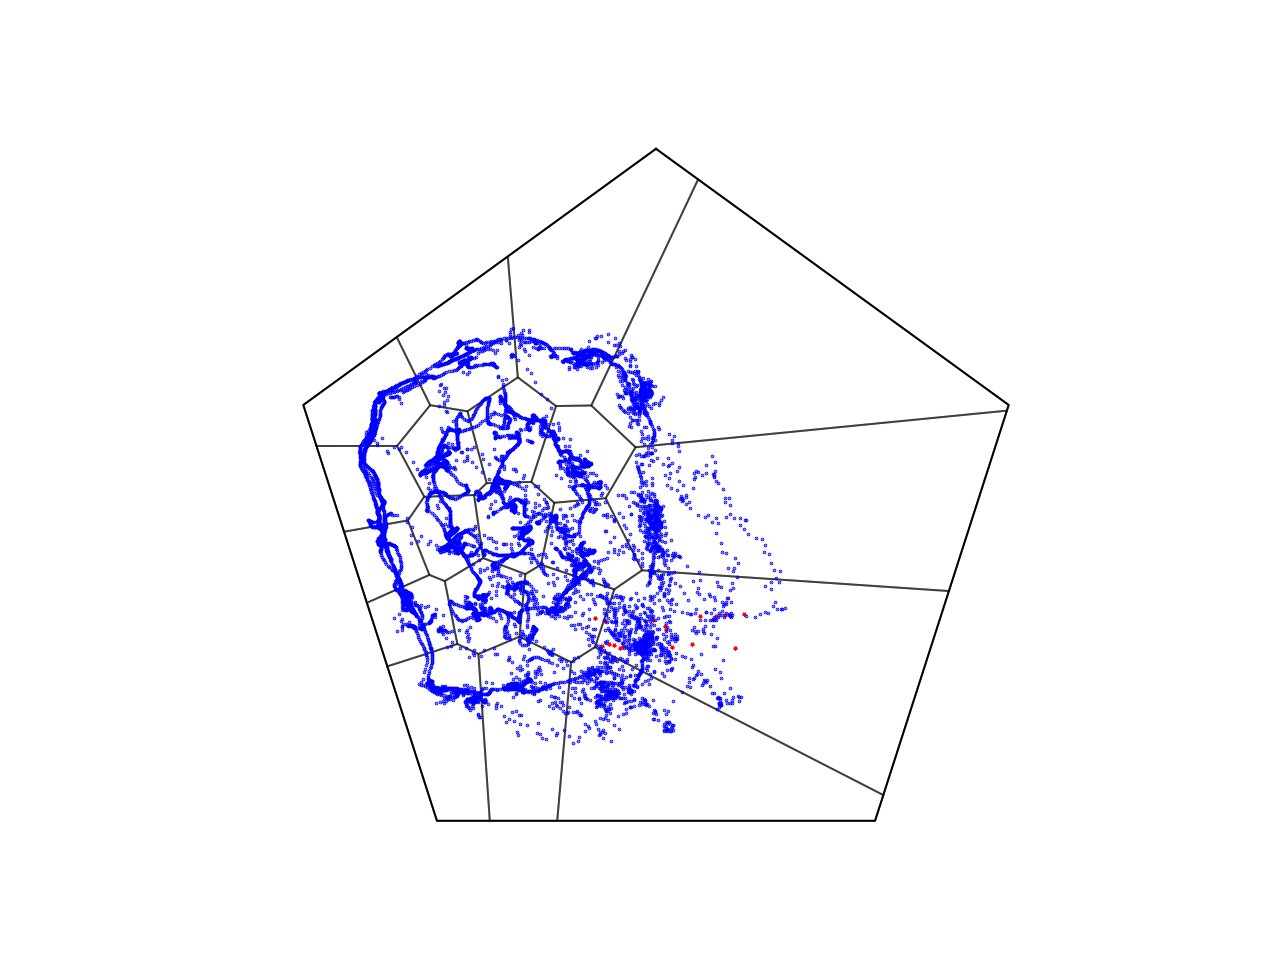
\includegraphics[scale=.2]{poster_sim1_tracking}
	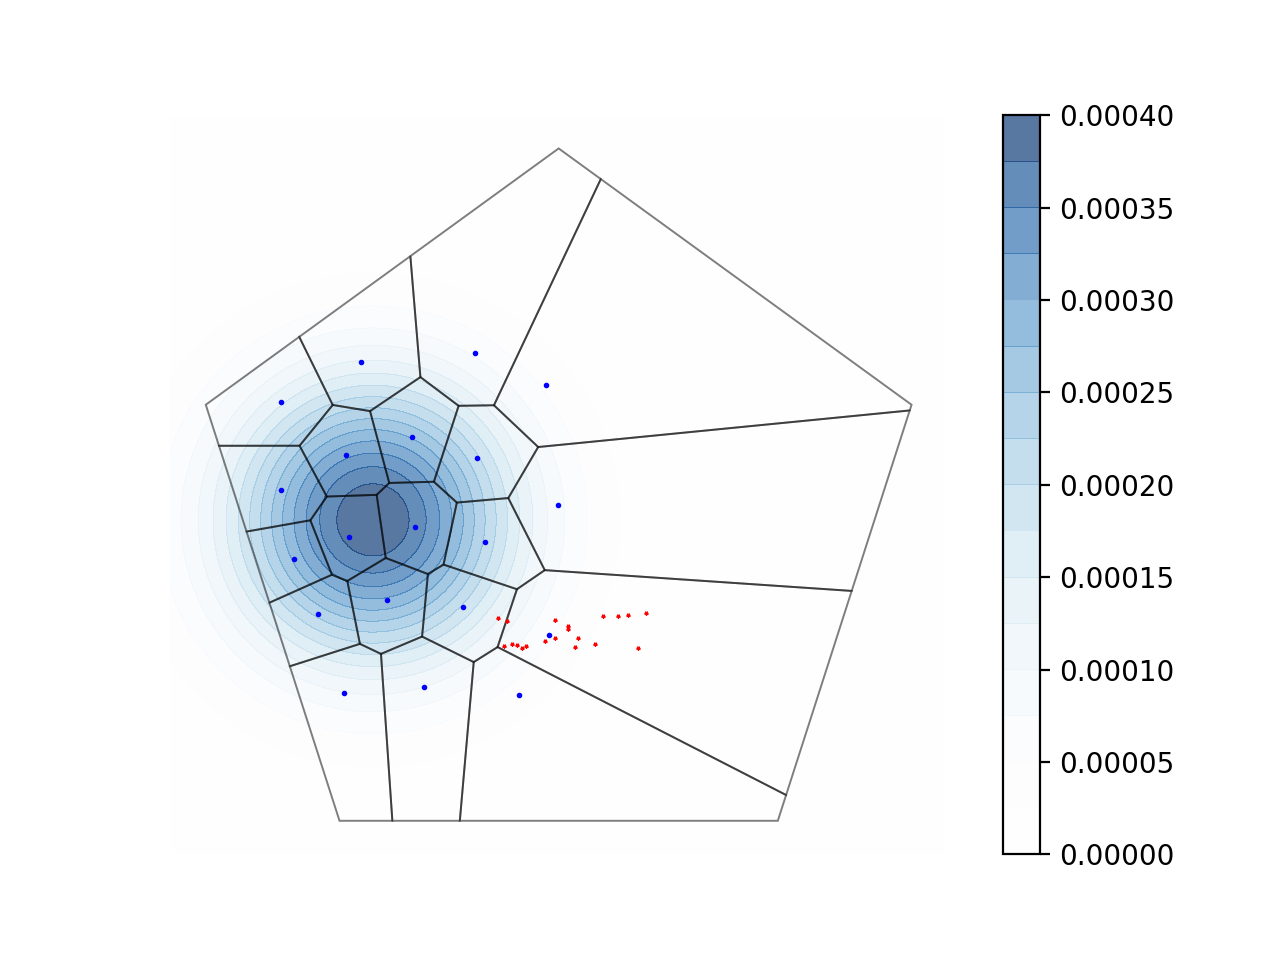
\includegraphics[scale=.2]{poster_sim1_final}
	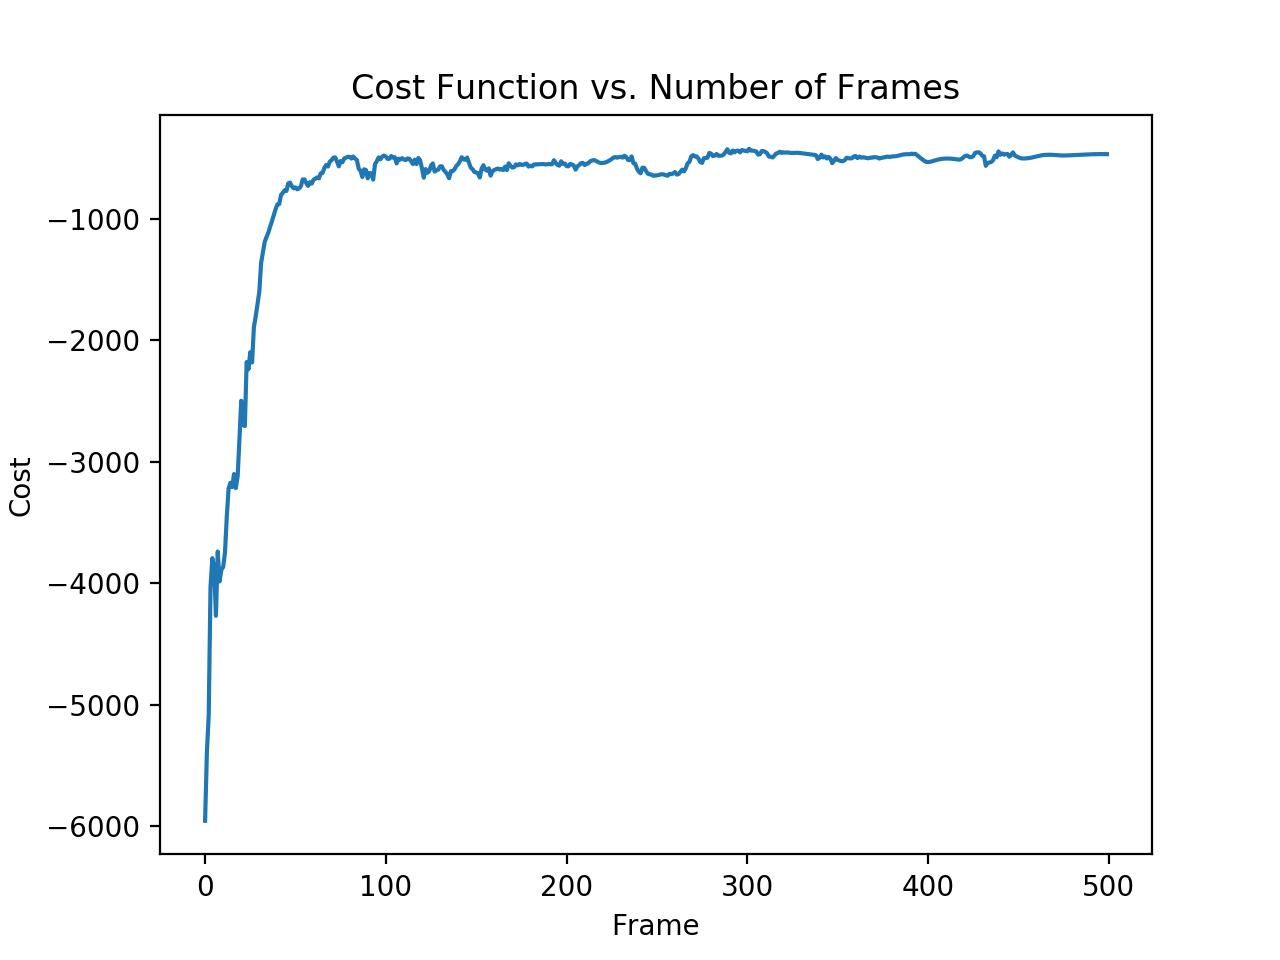
\includegraphics[scale=.2]{poster_sim1_cost_}
	\captionof{figure}{Scenario 1: The position of the agents is tracked (top left), with the red dot denoting the starting point. The final configuration of the agents is also shown (top right). The cost function $\mathcal{H}$ as a function of the number of frames (bottom center). The dark blue area is a Gaussian of covariance $\sigma_x = \sigma_y = 20$ and is centered at $(-50, 0)$.}
\end{center}
\begin{center}
	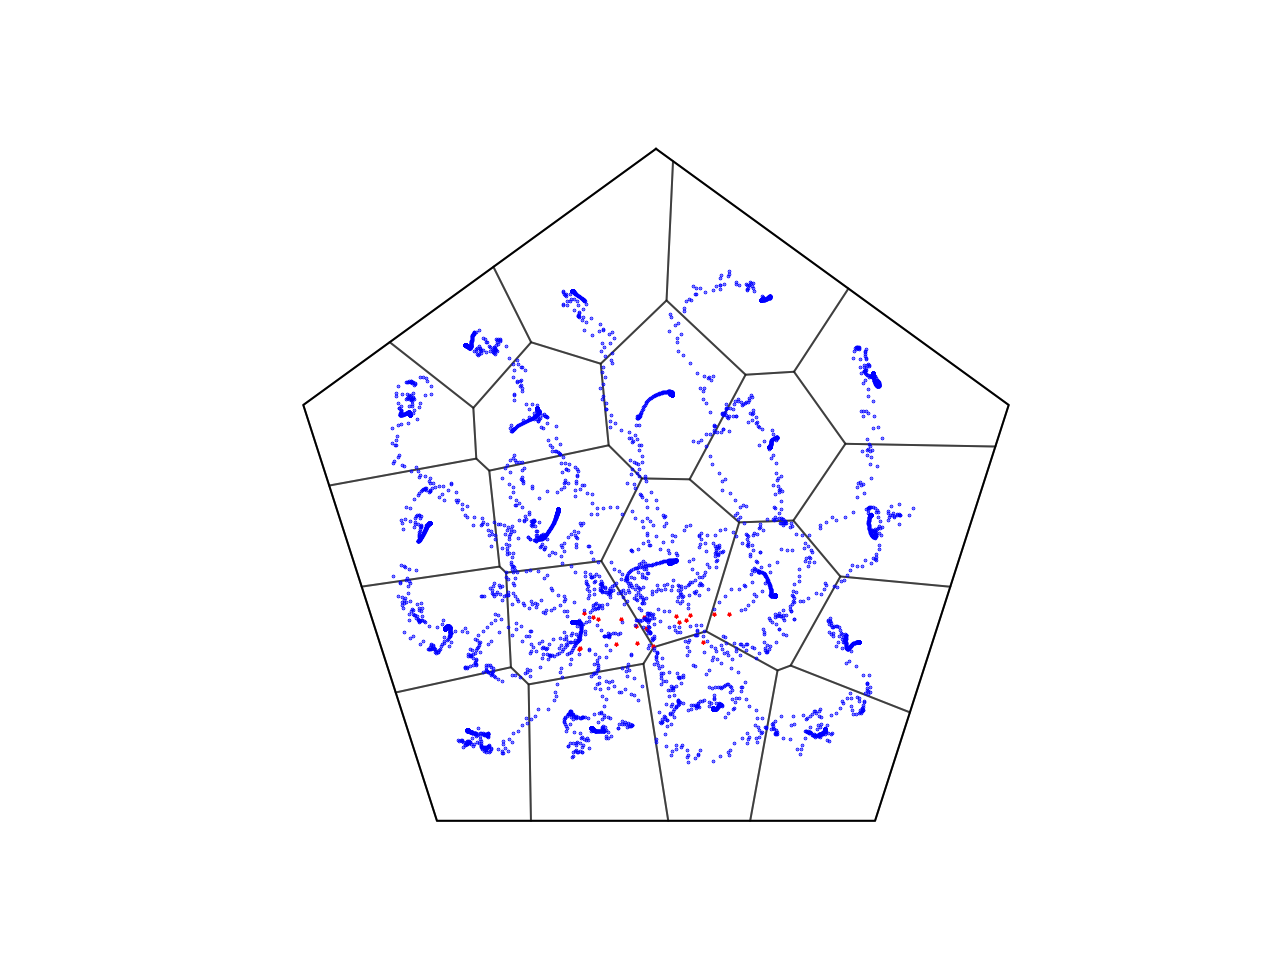
\includegraphics[scale=.2]{poster_sim2_tracking}
	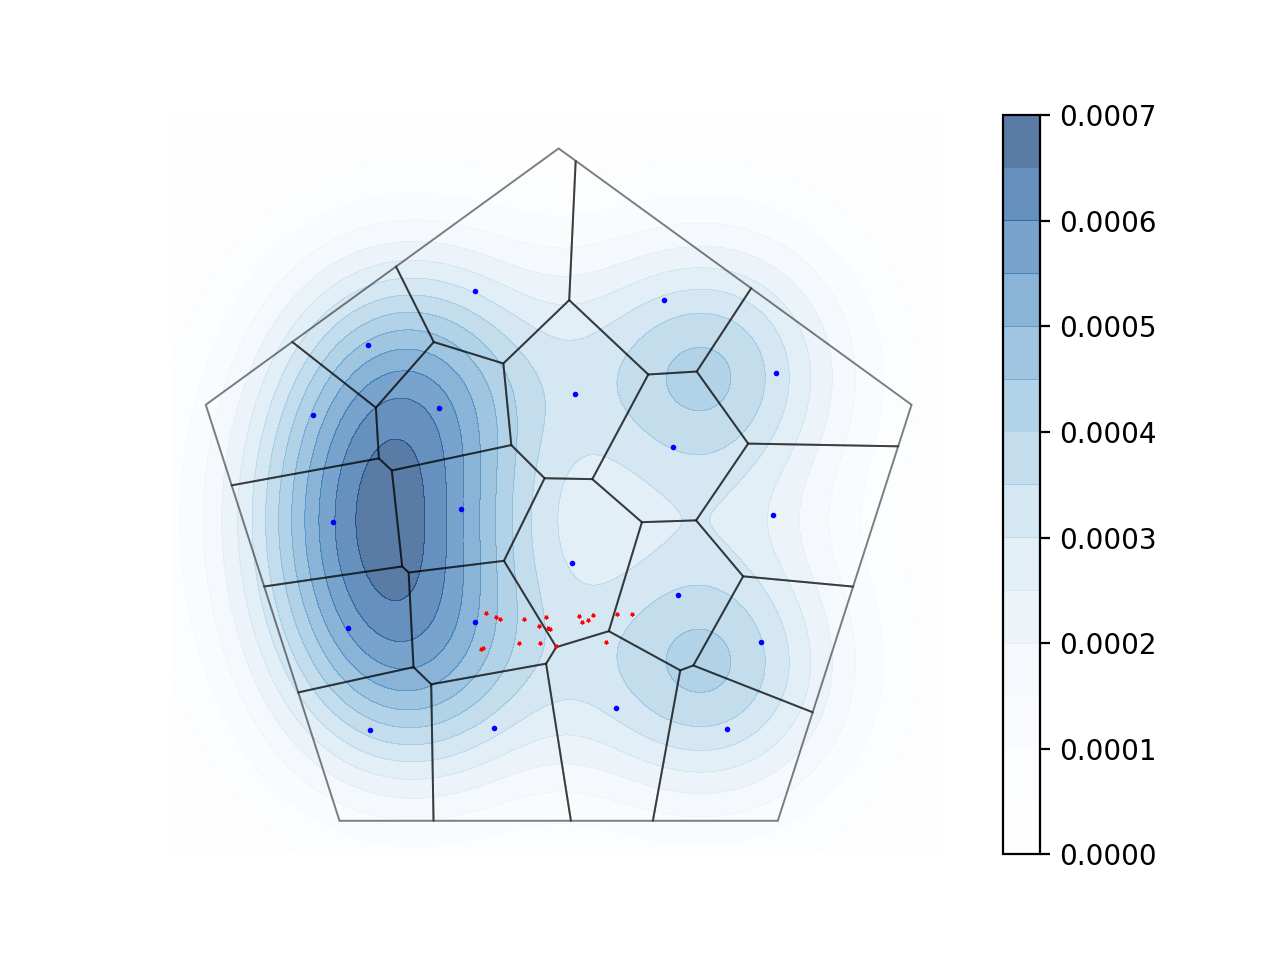
\includegraphics[scale=.2]{poster_sim2_final}
	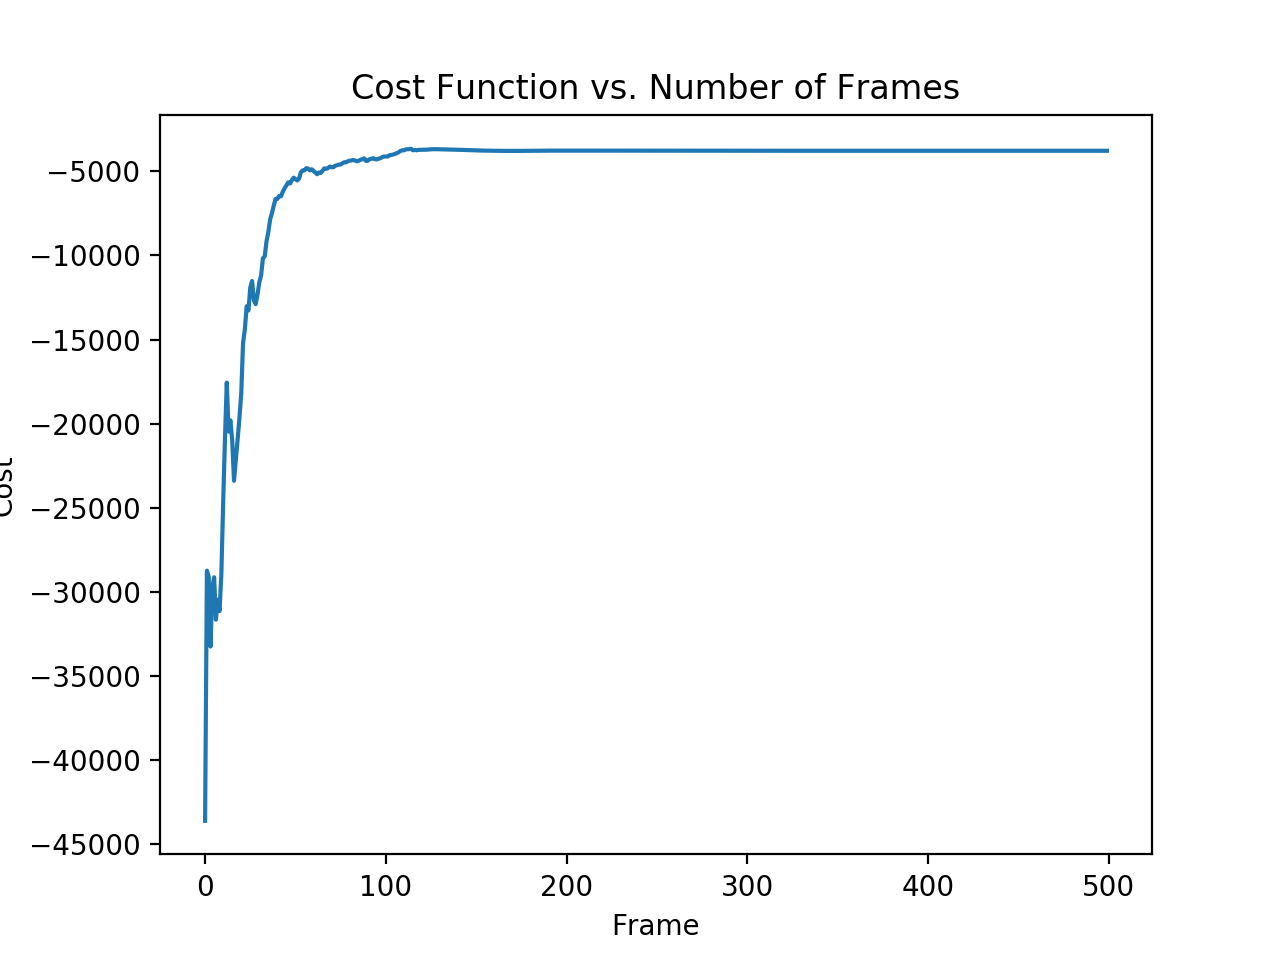
\includegraphics[scale=.2]{poster_sim2_cost_}
	\captionof{figure}{Scenario 2: The position of the agents is tracked (top left), with the red dot denoting the starting point. The final configuration of the agents is also shown (top right). The cost function $\mathcal{H}$ as a function of the number of frames (bottom center). The dark blue areas are Gaussians of covariance $\sigma_x = \sigma_y = 20$ and are centered at $(-50, 0), (-40,40), (-40,-40), (40,-40), (40,40)$.}
\end{center}
\begin{center}
	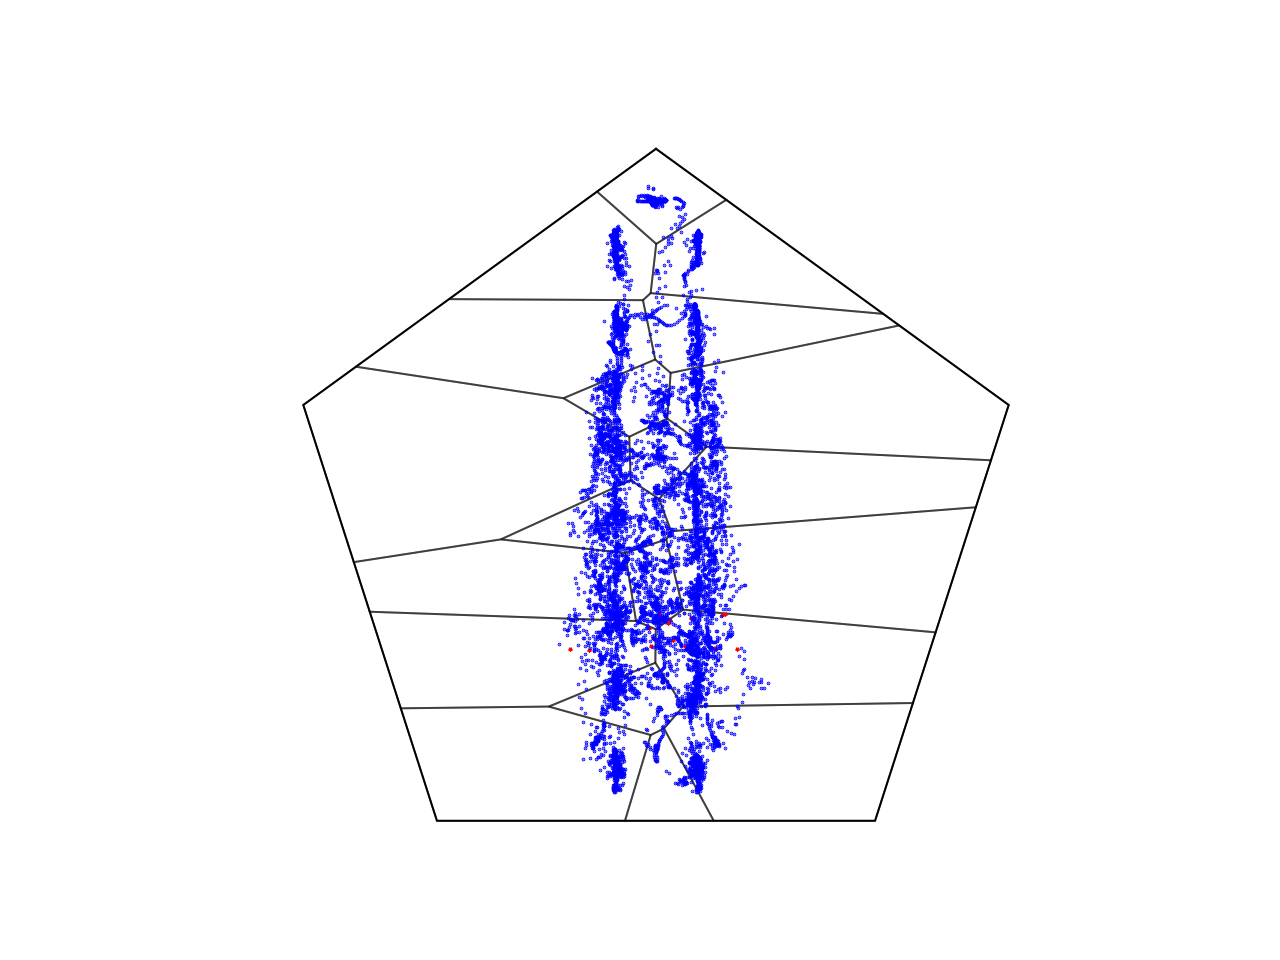
\includegraphics[scale=.2]{poster_sim3_tracking}
	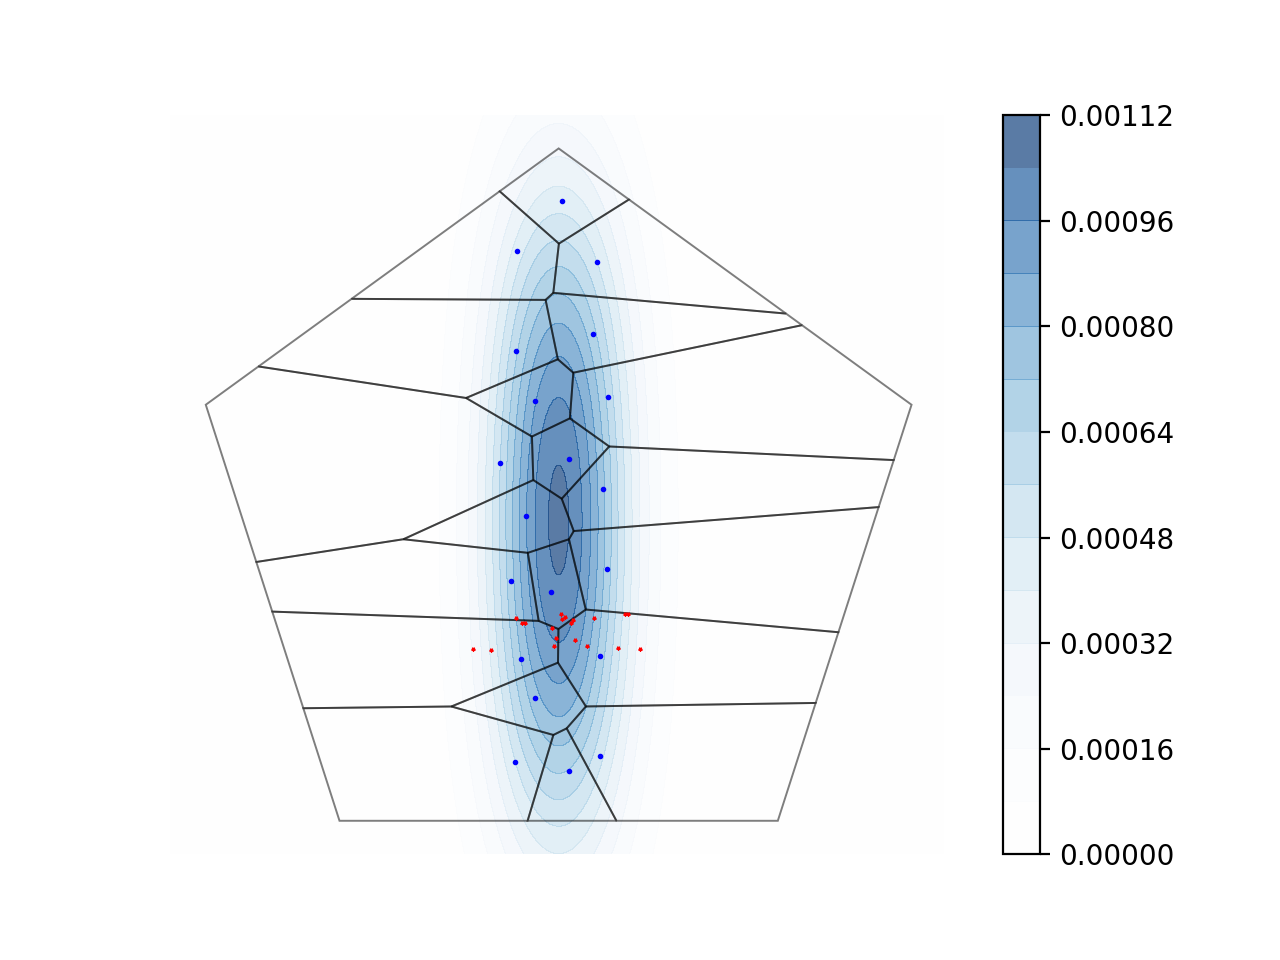
\includegraphics[scale=.2]{poster_sim3_final}
	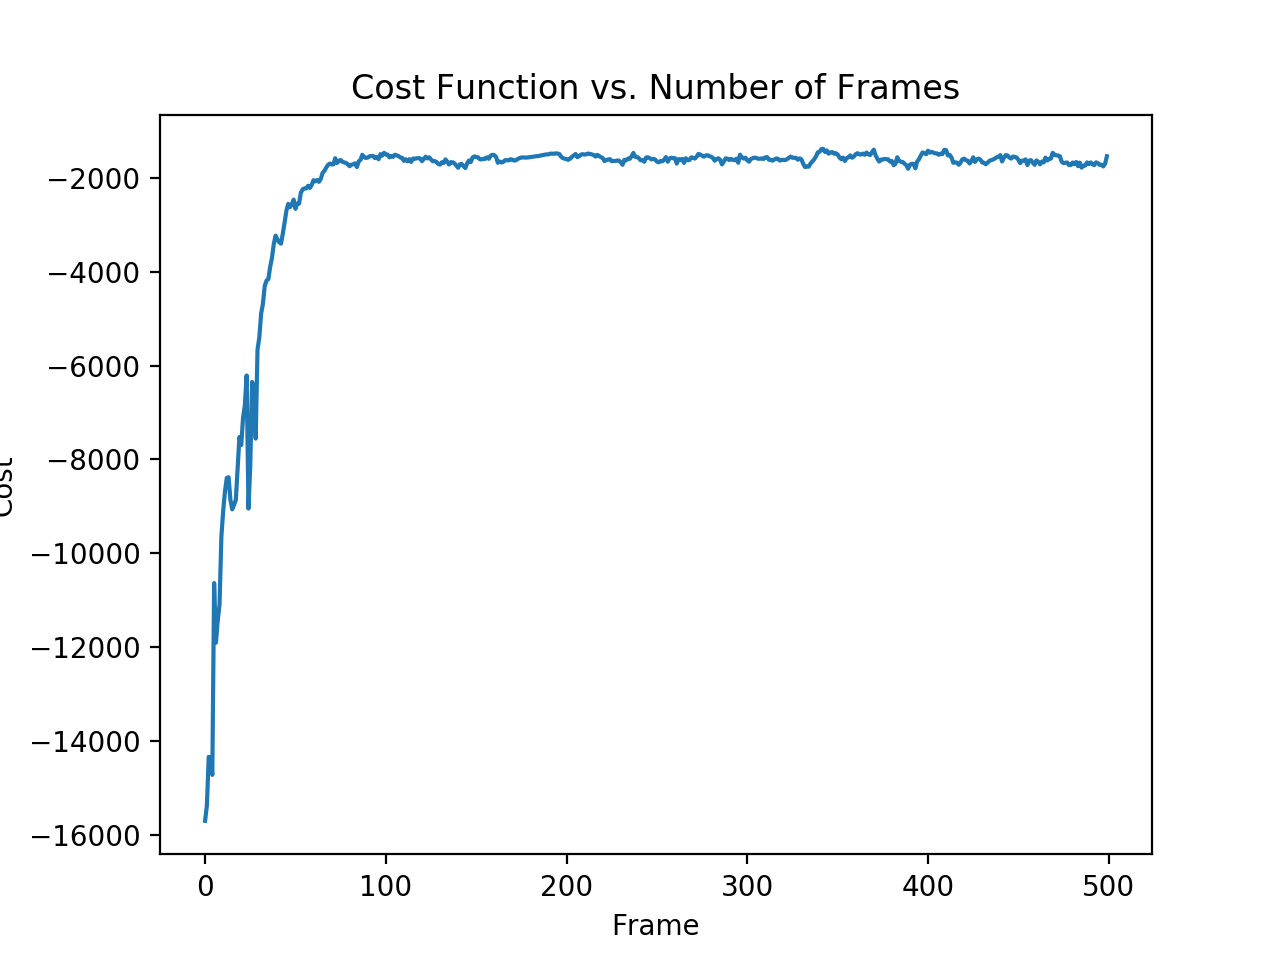
\includegraphics[scale=.2]{poster_sim3_cost_}
	\captionof{figure}{Scenario 3: The position of the agents is tracked (top left), with the red dot denoting the starting point. The final configuration of the agents is also shown (top right). The cost function $\mathcal{H}$ as a function of the number of frames (bottom center). The dark blue areas are Gaussians of covariance $\sigma_x = 10, \sigma_y = 30$ and are centered at $(0,0), (0,50), (0,-50)$.}
\end{center}
\section{Further Discussion}
The simulation results show that the proposed area coverage control law does indeed provide enough coverage of the domain. However, the simulations do not show the true power of the algorithm. The reason we turned to reinforcement learning methods was because traditional control methods perform poorly at worst, and adequately at best, when the environment is dynamic or the dynamics of the agents are highly nonlinear. Future areas of study would be to apply the area coverage control law to more complex environments and use more interesting dynamics. 

Additionally, the area coverage control law was distributed with respect to the Voronoi tesselation but not the TD3 algorithm. Better reinforcement learning methods like D4PG \cite{barth-maron2018distributional} and multi-agent deep deterministic policy gradients (MADDPG) \cite{lowe2017multiagent} are more suited for the multi-agent case especially when the agents must cooperate with each other to perform specific tasks. 

Finally, the $\phi$ that is used has to be learned by some external algorithm. In the simulations, we used faux examples of $\phi$ that are reasonable for simulation but unrealistic in nature. 
\section{Conclusion}
	In this paper, an area coverage control law in cooperation with a reinforcement learning technique was proposed for solving the optimal deployment problem. A delayed actor-critic deep deterministic policy gradient (TD3) algorithm is proposed to learn the value function and policy. Simulation results were presented for stationary and time-varying scalar fields. The simulation results show that the algorithm is efficient for solving the area coverage control problem, though with simple dynamics. 
\nocite{*}
\bibliography{ref}
\bibliographystyle{ieeetr}
	
\end{document}